
%% !TEX root = manual.tex

\section{Spyplot Diagrams}
\label{sec:tutorials:spyplot}

Spyplots visualize communication matrices, showing either the number of messages or number of bytes sent between two network endpoints.
They are essentially contour diagrams, where instead of a continuous function $F(x,y)$ we are plotting the communication matrix $M(i,j)$.
An example spyplot is shown for a simple application that only executes an MPI\_Allreduce (Figure \ref{fig:spyplot}).
Larger amounts of data (red) are sent to nearest neighbors while decreasing amounts (blue) are sent to MPI ranks further away.

\begin{figure}[h]
\centering
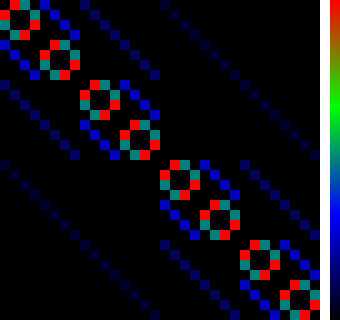
\includegraphics[width=0.4\textwidth]{figures/spyplot/mpi_spyplot.png}
\caption{Spyplot of Bytes Transferred Between MPI Ranks for MPI\_Allreduce}
\label{fig:spyplot}
\end{figure}

Various spyplots can be activated by boolean parameters in the input file.
The most commonly used are the MPI spyplots, for which you activate the spyplot as part of the MPI subcomponent.

\begin{ViFile}
node {
  app1 {
    mpi {
      traffic_matrix {
        fileroot = test
      }
    }
  }
}
\end{ViFile}

After running there will be a .csv and .png file in the folder, with e.g. \inlineshell{fileroot = test}

\begin{ShellCmd}
example> ls 
test.png
test.csv
\end{ShellCmd}
\inlineshell{test.png} shows the number of bytes exchanged between MPI ranks.
To extend the analysis you can instead specify as part of the NIC subcomponent

\begin{ViFile}
node {
  nic {
    traffic_matrix {
      fileroot = test
    }
  }
}
\end{ViFile}
A new csv/png will appear showing the number of bytes exchanged between physical nodes, 
accumulating together all MPI ranks sharing the same node.
This gives a better sense of spatial locality when many MPI ranks are on the same node.


